\documentclass[10pt,a4paper,twoside]{article}

\usepackage[utf8]{inputenc}
\usepackage[francais]{babel}
\usepackage[T1]{fontenc}
\usepackage{amsmath}
\usepackage{amsfonts}
\usepackage{amssymb}
\usepackage{graphicx}
\usepackage{placeins}
\usepackage{lscape}

\author{Victor Lezaud}
\title{Cours Architecture de circuit numérique}
\begin{document}

\maketitle
\renewcommand{\contentsname}{Sommaire}
\tableofcontents

\newpage

\section{Le binaire}

\subsection{Nombre en base 2}
\subsubsection{Entiers naturels en base 2}
En base 2 les entiers naturels ne sont définis que par des 1 et des 0. Comme en base 10, on use de notation positionnelle : il faut multiplier chaque chiffre par $2^{n}$ avec $n$ le nombre de chiffre avant lui.\\
Soit $x$ un nombre codé sur $n$ bits, noté $x_{i}$ : $x = \sum_{i=0}^{n}x_{i} \times 2^{i}$
\subsubsection{Valeurs importantes}
Il est important de retenir quel est le maximum que l'on peut stocker en un certain nombre de bits:
\begin{itemize}
\item 8 bits : $255$
\item 10 bits : $\sim 10^{3}$
\item 16 bits : $65.000$
\item 32 bits : $\sim 4\times 10^{9}$
\end{itemize}

\subsubsection{Entier relatif : complément à 2}
\paragraph{Première idée :} Dans un ordinateur on ne peut enregistrer que des 1 et des 0 alors comment noter des entiers relatifs? L'une des solutions serait d'utiliser par exemple le bit de poids fort pour définir le signe (0 pour plus et 1 pour moins). Le problème de cette méthode est qu'elle implique de redéfinir les opérations pour les nombres négatifs.

\paragraph{Le complément à 2} permet de garder les mêmes opérations pour les nombre positifs et négatifs. L'appellation complément à 2 est un abus de langage on devrait dire complément à $2^{n}$ avec n le nombre de bits utilisé. En effet la définition du complément à $2^{n}$ est que $x-x$ donne $2^{n}$ en binaire (soit un 1 suivi de n 0) ce qui rapporté à n bits vaut 0. 
% Ainsi on code $-1$ de manière à ce que $-1+1=0$ et cela donne 4 bits $1111 + 1 = 0000$ ou encore $-3+3=0$ soit $1101+0011=0000$.

\begin{figure}[hbtp]
\caption{Complément à 2 sur 4 bits}
\centering
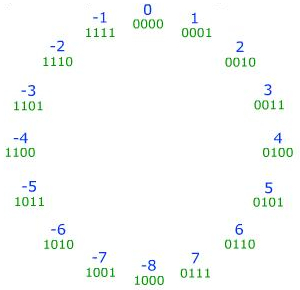
\includegraphics[scale=0.5]{cercleBinaire.jpg}
\end{figure}

\paragraph{L'opposé :} est obtenu simplement en complément à 2 : on inverse tous les chiffres et on ajoute 1. Par exemple $-3=-(0011)=1100+1=1101$

\subsection{Conversion}
\subsubsection{Binaire -> décimal}
\paragraph{Entier positif :} Soit $x$ un nombre codé sur $n$ bits, noté $x_{i}$ : $x = \sum_{i=0}^{n}x_{i} \times 2^{i}$. Chaque 1 ajoute donc $2^{n}$ avec $n$ le nombre de chiffres après.

\paragraph{Parité et signe :} En binaire on peut voir directement le signe d'un nombre (en codage en complément à 2) avec son bit de poids fort (0 positif, 1 négatif) et sa parité avec le bit de poids faible (0 pair, 1 impair).

\paragraph{Entier négatif :} Il n'y a pas de conversion simple entre la base 2 et la base 10 pour les entiers négatifs. On prend donc l'opposé puis on convertit en base 10 et on ajoute le signe.

\subsubsection{Décimal -> binaire}
\paragraph{Entier positif :} On effectue la division euclidienne du nombre, le reste donne le premier bit et on recommence avec le quotient pour obtenir le deuxième bit et ainsi de suite jusqu'à obtenir un quotient nul. Exemple : \\
 
\paragraph{Entier négatif:} De même pour passer du décimal et binaire d'un nombre négatif il faut prendre l'opposé puis faire la conversion et reprendre l'opposé.

\newpage
\section{Combinatoire}

\subsection{Calcul booléen}
\subsubsection{Base de l'algèbre booléenne}
\paragraph{Valeur booléenne :} Les valeurs booléenne n'ont que deux valeur possible $VRAI=1$ ou $FAUX=0$. Cela correspond à un bit dans un ordinateur.

\paragraph{Fonctions booléennes :} L'algèbre booléenne possède trois opérations :
\begin{itemize}
\item La négation est une opération unaire, notée $NOT(a) = \neg a = \bar{a}$
\item La disjonction est une opération binaire, notée $OR(a,b) = a \vee b = a+b$, 0 est élément neutre.
\item La conjonction est une opération binaire, notée $AND(a,b) = a \wedge b = ab$, 1 est élément neutre
\end{itemize}

\subsubsection{Règle de calcul}
\begin{tabular}{lcr}
Absorption & $a+1=1$ & $a\cdot 0 = 0$ \\ 
Elt neutre & $a+0=a$ & $a\cdot 1 = a$ \\ 
Idempotence & $a+a=a$ & $aa = a$ \\ 
Tautologie/Antilogie & $a+\bar{a}=1$ & $a \bar{a} = 0$ \\ 
Distributivité & $a+(bc) = (a+b)(a+c)$ & $a(b+c) = ab+ac$ \\ 
Associativité & $a+(b+c) = (a+b)+c$ & $(ab)c = a(bc)$ \\ 
De Morgan & $\overline{a+b} = \bar{a} \cdot \bar{b}$ & $\overline{ab} = \bar{a} + \bar{b}$ \\ 
\end{tabular} 

\subsubsection{Expression booléenne}
La combinaison de variables booléennes grâce aux 3 opérateurs forme une expression booléenne qui renvoie une valeur booléenne en fonction des autres valeurs. Une expression booléenne avec $n$ variables crée une fonction de $\mathbb{B}^{n}$ à $\mathbb{B}$. Il faut donc $m$ expressions pour créer une fonction $\mathbb{B}^{n}$ à $\mathbb{B}^{m}$.

\subsubsection{Table de vérité}
\begin{tabular}{c|c||c|c|c}
$a$ & $b$ & $\bar{a}$ & $a+b$ & $ab$ \\ 
\hline 
0 & 0 & 1 & 0 & 0 \\ 
0 & 1 & 1 & 1 & 0 \\ 
1 & 0 & 0 & 1 & 0 \\ 
1 & 1 & 0 & 1 & 1 \\ 
\end{tabular} 

\subsection{Circuit combinatoire}
\subsubsection{Porte logiques}
Il existe une porte logique pour chacune des opérations de l'algèbre booléenne. Les portes logiques permettent de réaliser les expressions booléennes.

\begin{figure}[hbtp]
\caption{Porte logique élémentaire}
\centering
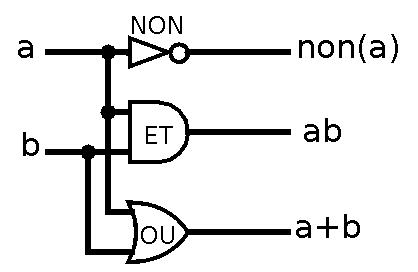
\includegraphics[scale=0.33]{PorteLogique.jpg}
\end{figure}
\FloatBarrier

\subsubsection{Règle d'assemblage}
Un Circuit Logique Combinatoire est :
\begin{itemize}
\item Une porte
\item Un fil
\item Deux CLC connecté entre eux
\end{itemize}
Il est interdit de :
\begin{itemize}
\item créer des cycles
\item connecter des sorties ensembles
\end{itemize}

\subsubsection{Multiplexeur}
\paragraph{Principe :} Un multiplexeur de $n$ vers $1$ permet de choisir laquelle des $n$ entrées donne sa valeur à la sortie. Un démultiplexeur de $1$ vers $n$ permet de choisir laquelle des sorties récupère la valeur de l'entrée.


\begin{table}[hbtp]
	\caption{Table de vérité de multiplexeur 2 vers 1}
	\centering
	\begin{tabular}{c|c|c||c}
		E0 & E1 & choix & Sortie \\ 
		\hline 
		0 & 0 & 0 & 0 \\ 
		0 & 1 & 0 & 0 \\ 
		1 & 0 & 0 & 1 \\ 
		1 & 1 & 0 & 1 \\ 
		0 & 0 & 1 & 0 \\ 
		0 & 1 & 1 & 1 \\ 
		1 & 0 & 1 & 0 \\ 
		1 & 1 & 1 & 1 \\ 
	\end{tabular}
\end{table}

\begin{table}[hbtp]
	\caption{Table de vérité de démultiplexeur 1 vers 2}
	\centering
	\begin{tabular}{c|c||c|c}
	Entrée & choix & S0 & S1 \\ 
	\hline 
	0 & 0 & 0 & 0 \\ 
	1 & 0 & 1 & 0 \\ 
	0 & 1 & 0 & 0 \\ 
	1 & 1 & 0 & 1 \\ 
	\end{tabular} 
\end{table}

\begin{figure}[hbtp]
\caption{Circuit numérique multiplexeur 2 vers 1}
\centering
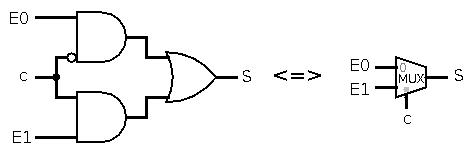
\includegraphics[scale=0.5]{Mult2vers1.jpg}
\end{figure}

\begin{figure}[hbtp]
\caption{Circuit numérique démult 1 vers 2}
\centering
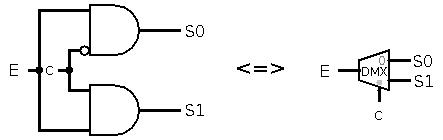
\includegraphics[scale=0.5]{Mult1vers2.jpg}
\end{figure}

\paragraph{Réalisation :} A partir des tables de vérité, on peut déduire les expression booléennes suivantes, à partir des quelles on construits les circuits combinatoires:
\begin{itemize}
\item Multiplexeur 2 vers 1 : $s = e_{0}\bar{c} + e_{1}c$
\item Multiplexeur 1 vers 2 : $s_{0} = e\bar{c} \ et\ s_{1} = ec$
\end{itemize}

\FloatBarrier
\newpage
\section{Mémoire}
\subsection{But}
Jusqu'à maintenant nous avons réalisé que des circuits combinatoires qui associent toujours les mêmes sorties aux mêmes entrées quelque soient les entrées précédentes. Mais la plupart du temps on veut que l'automate réagisse différemment en fonction de ce qu'il s'est passé avant.

\subsection{Réalisation de la mémoire}
\paragraph{Principe :} On cherche à stocker un bit en mémoire, c'est à dire quand on veut pouvoir fixer la valeur à stocker par le circuit et le circuit doit renvoyer cette valeur jusqu'à ce qu'on décide de la changer.\\
\paragraph{Verrou :} Un verrou permet de stocker un bit grâce à un multiplexeur 2 vers 1. Une entrée permet d'envoyer la valeur à stocker et l'autre est branchée sur la sortie. Le bit de sélection permet de choisir si on veut modifier ou non la valeur stocker\\

\begin{figure}[hbtp]
\caption{Verrou}
\centering
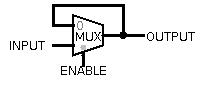
\includegraphics[scale=1]{Verrou.jpg}
\end{figure}
\FloatBarrier

\subsubsection{Clock}
Aujourd'hui 99\% des circuits numériques sont synchrones. Un circuit synchrone est basé sur une horloge (ou CLOCK). Cela permet de masquer les délais de propagation.\\
Les circuits séquentiels ne s'actualisent qu'à des instants précis définis par des fronts montants (ou descendants) de l'horloge

\subsubsection{Registre}
\paragraph{Le problème du verrou :} Le verrou qu'on a vu plus haut n'est malheureusement pas synchrone. On va donc chercher maintenant à créer une mémoire synchrone.

\paragraph{Bascule synchrone :} Le Flip-Flop permet de créer une bascule synchrone, c'est-à-dire que la valeur de la sortie est toujours égale à la valeur de l'entrée au dernier top d'horloge.

\begin{figure}[hbtp]
\caption{Flip-Flop}
\centering
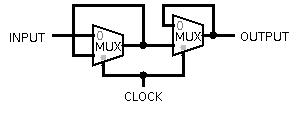
\includegraphics[scale=1]{FlipFlop.jpg} 
\end{figure}
\FloatBarrier

\paragraph{Flip-Flop + Verrou :} En mettant un verrou avant un Flip-Flop, on rend le verrou synchrone et cela permet bien de stocker une valeur de manière synchrone. On a donc un circuit qui permet de stocker l'entrée au top d'horloge si $ENABLE=1$ et de la garder jusqu'à ce qu'on la modifie à un autre top d'horloge.

\begin{figure}[hbtp]
\caption{Flip-Flop avec enable}
\centering
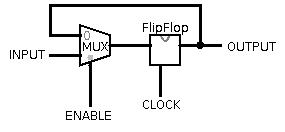
\includegraphics[scale=1]{FlipFlopEnable.jpg} 
\end{figure}
\FloatBarrier

\paragraph{Dernière étape :} Pour finir notre registre 1bit on ajoute une entrée RESET pour remettre à zéro le registre. Donc voici comment réaliser un registre :

\begin{figure}[hbtp]
\caption{Registre}
\centering
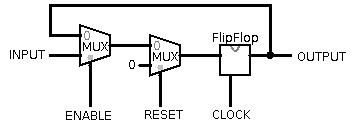
\includegraphics[scale=1]{Registre.jpg}
\end{figure}
\FloatBarrier

\paragraph{Registre n bits :} Pour réaliser un registre à n bits il suffit de mettre n registre à 1bit côte à côte. Chaque bit d'entrée est lié à un des registre à 1bit et de même pour les sorties. On lie les RESET et ENABLE pour qu'il soit géré par un seul bit.

\subsection{Machine à Etat Fini}
\subsubsection{Définition}
\paragraph{Une Machine à État Fini} est un tuple  $(Q,q_{0},I,T)$ avec:
\begin{itemize}
\item $Q$ est l'ensemble des états
\item $q_{0} \in Q$ est l'état initial
\item $I$ est l'alphabet d'entrées
\item $T \subseteq Q\times I\times Q$ est la fonction de transition
\end{itemize}

\paragraph{Et les sorties ?} En effet en l'état la machine n'a aucune sortie et donc ne communique aucun résultat. Il y a deux manières d'ajouter les sorties:
\begin{itemize}
\item Lors des transitions : Machine de Mealy
\item Lors des états : Machine de Moore
\end{itemize}


\subsubsection{Automates de Mealy et de Moore}
\paragraph{Un automate de Mealy} est un tuple  $(Q,q_{0},I,O,T)$ avec:
\begin{itemize}
\item $Q$ est l'ensemble des états
\item $q_{0} \in Q$ est l'état initial
\item $I$ est l'alphabet d'entrées
\item $T \subseteq Q\times I\times O \times Q$ est la fonction de transition
\end{itemize}

\paragraph{Un automate de Moore} est un tuple  $(Q,q_{0},I,O,T)$ avec:
\begin{itemize}
\item $Q$ est l'ensemble des états
\item $q_{0} \in Q$ est l'état initial
\item $I$ est l'alphabet d'entrées
\item $T \subseteq Q\times I\times Q$ est la fonction de transition
\item $F \subseteq Q \rightarrow O$ est une fonction de sortie
\end{itemize}

\paragraph{Mealy ou Moore :} Les deux sont équivalents mais Mealy représente plus un aspect événementiels. En architecture des ordinateurs on utilise plus Moore.

\subsubsection{Exemple}
Dans cet exemple On réalise un automate qui renvoie 1 s'il reçoit au moins 4 fois 1 d'affilée et 0 sinon.

\begin{figure}[hbtp]
\caption{Exemple d'automate de Moore}
\centering
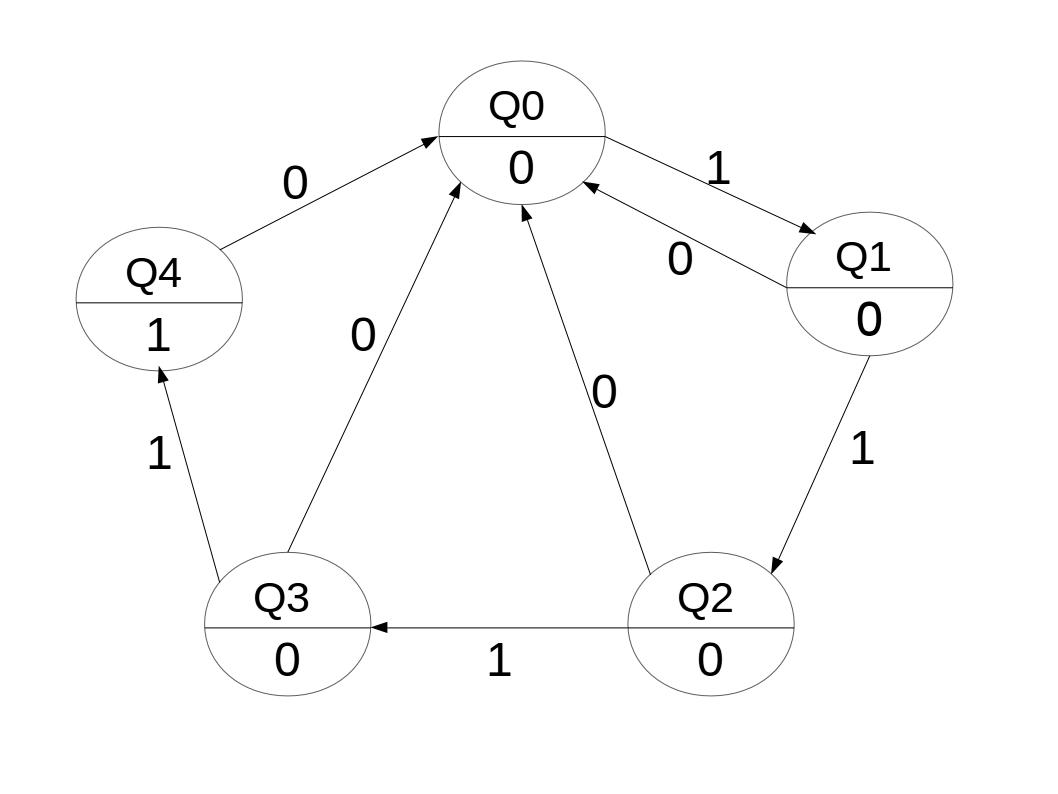
\includegraphics[scale=0.2]{Moore.jpg}
\end{figure}
\FloatBarrier

Pour décrire le fonctionnement d'une machine de Moore il suffit de représenter la fonction de transition est la fonction de sortie:

\begin{tabular}{c|ccc}
T & Q & I & Q \\ 
\hline 
 & 0 & 0 & 0 \\ 
 & 0 & 1 & 1 \\ 
 & 1 & 0 & 0 \\ 
 & 1 & 1 & 1 \\ 
 & 2 & 0 & 0 \\ 
 & 2 & 1 & 1 \\ 
 & 3 & 0 & 0 \\ 
 & 3 & 1 & 1 \\ 
\end{tabular} 
\begin{tabular}{c|cc}
S & Q & O \\ 
\hline 
 & 0 & 0 \\ 
 & 1 & 0 \\ 
 & 2 & 0 \\ 
 & 3 & 1 \\ 
\end{tabular} 

\subsubsection{Séparation du contrôle et des données}
\paragraph{Limite de la machine de Moore :} Reprenons l'exemple précédent et imaginons que nous voulions attendre 100 tops d'horloge. Il faudrait créer 100 états différents.

\paragraph{Séparation du contrôle et des données :} Pour régler le problème on sépare le contrôle (effectué par l'automate) et les données. Ainsi de 100 états on passe à 3. Certains problèmes ne peuvent être résolu que de cette manière.

\subsubsection{Schéma de l'automate de Moore avec séparation des données}

\begin{figure}[hbtp]
\caption{L'automate de Moore}
\centering
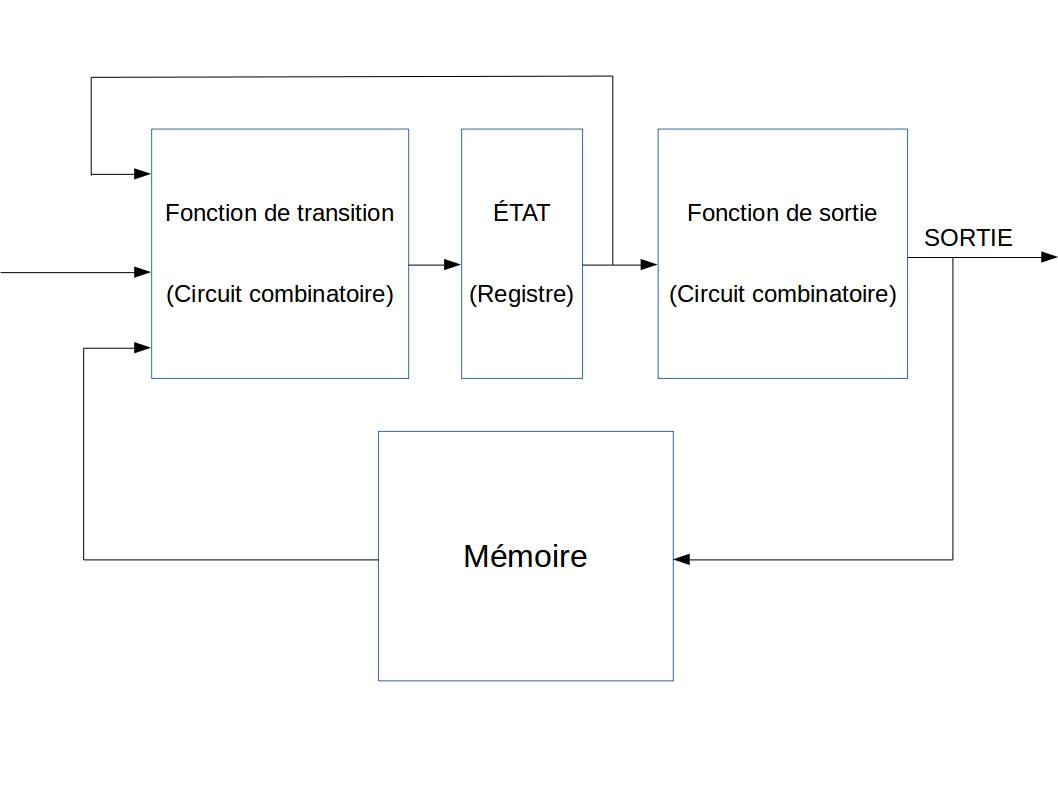
\includegraphics[scale=0.33]{SchemaMachineMoore.jpg} 
\end{figure}
\FloatBarrier

\newpage
\section{Machine de Von Neumann}

\subsection{Problème}
\paragraph{Jusque là} nous avons créé des automates qui réalise toujours un objectif bien précis. Ils exécutent toujours le même algorithme, on crée d'ailleurs l'automate dans l'unique but de réaliser un algorithme bien précis.

\paragraph{Un ordinateur} est fondamentalement différent car il réalise des algorithmes qui sont stockés dans la mémoire. On a donc besoin d'une organisation et d'un automate beaucoup plus flexible. L'ensemble des ordinateurs modernes sont basés sur la machine de Von Neumann qui permet de résoudre ces problèmes.

\subsection{Divide et Impera}
\begin{figure}[hbtp]
\caption{Architecture d'une machine de Von Neumann}
\centering
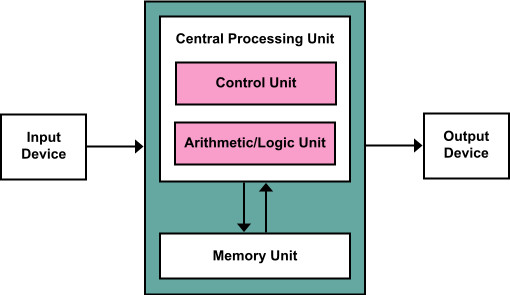
\includegraphics[scale=0.5]{Von_Neumann_Architecture.jpg}
\end{figure}

\subsubsection{Présentation}
L'organisation de la Machine de Von Neumann sépare au maximum les tâches à effectuer, elle est composée de trois éléments:
\begin{itemize}
\item La mémoire
\item L'automate de contrôle
\item L'unité de calcul (Arithmetic Logic Unit et Datapath)
\end{itemize}

\subsubsection{La mémoire}
La mémoire stocke toutes les données de l'ordinateur. C'est ici que se trouvent les programmes exécutés par la machine.

\subsubsection{L'automate de contrôle}
\paragraph{Principe :} L'automate de contrôle est le seul à savoir ce qui doit être fait et quand cela doit être fait et il doit activer les autres. Il ne sait faire absolument aucun traitement et ne stocke que son état actuel mais il est le seul à pouvoir activer tout le reste de la machine.
\paragraph{I/O :}Ses entrées sont l'instruction en cours, les rapports de l'unité de calcul, son état actuel et les entrées de l'utilisateur. Ses sorties sont les ordres pour l'unité de calcul et des sorties de la machine (ultrason de télémètre par exemple)

\paragraph{Cycle de Von Neumann :}
\begin{verbatim}
Boucle{
    Récupérer l'instruction
    Décoder l'instruction
    Executer l'instruction
    Aller à l'intruction suivante
}
\end{verbatim}

\begin{figure}[hbtp]
\caption{Cycle de Von Neumann en automate de Moore}
\centering
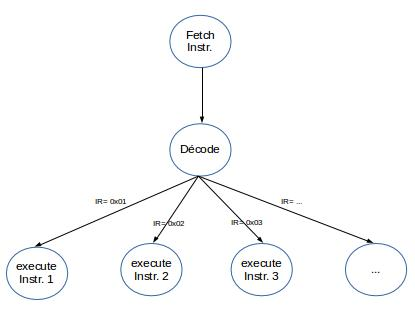
\includegraphics[scale=1]{cycle_automate_VN.jpg} 
\end{figure}
\FloatBarrier

\subsubsection{L'unité de calcul}
L'unité de calcul est la partie capable de traiter les données. Elle regroupe l'ensemble des calcul réalisable par l'ordinateur. Elle est pilotée par l'unité de contrôle qui grâce à des multiplexeurs va pouvoir sélectionner le calcul qui doit être envoyé en sortie.

\newpage
\subsubsection{En dessin}
\begin{figure}[hbtp]
\caption{Schéma détaillé de la machine de Von Neumann}
\centering
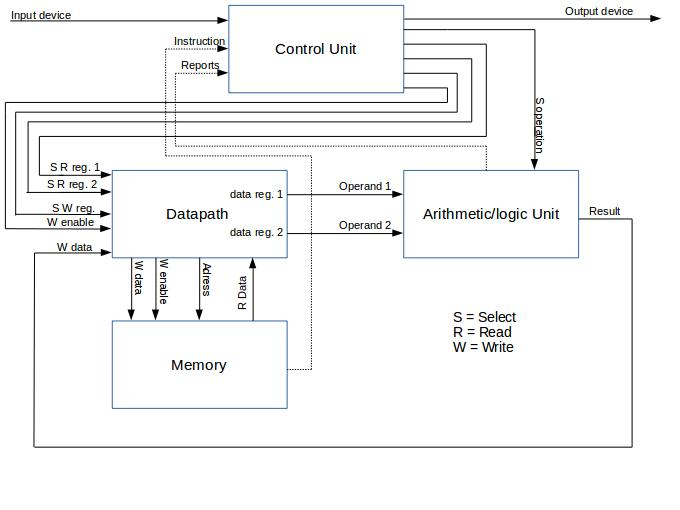
\includegraphics[scale=0.65]{MVN_detail.jpg} 
\end{figure}
\FloatBarrier


\end{document}
\grid
